\documentclass[a4paper,12pt]{article}
\usepackage{outline}
\usepackage{pmgraph}
\usepackage[normalem]{ulem}
\usepackage{comment} % enables the use of multi-line comments (\ifx \fi)
\usepackage{lipsum} %This package just generates Lorem Ipsum filler text.
\usepackage{fullpage} % changes the margin
\usepackage{listings}
\usepackage{color}
\usepackage{mdframed}
\usepackage{listings}
\usepackage{amssymb}
\usepackage{amsmath}
\usepackage{graphicx}
\graphicspath{ {../graphics/} }
\renewcommand{\lstlistingname}{Code Block}% Listing -> Algorithm
\renewcommand{\lstlistlistingname}{List of \lstlistingname s}% List of Listings -> List of Algorithms

\linespread{1.5}
%--------------------Indention
\setlength{\parindent}{15pt}
\lstset{frame=shadowbox, rulesepcolor=\color{white}}
\mdfsetup{frametitlealignment=\center}
\lstset{
  numbers=left,
  stepnumber=1,
  firstnumber=1,
  numberfirstline=true
}

\begin{document}
\section*{Objective}

  \hspace{15pt}The purpose of this lab is to further our knowledge of Verilog and circuit design by walking the student through the process of designing a combination lock. The lock is very similiar to the locks found on high school lockers. After building and designing a 3 digit lock, the student will then have to implement a 4-digit lock by modifying the existing design.

\section*{Design}
% combination lock fsm test
% 1.1.e Likewise, take a look at the simulation waveform and take note of the tests that the test bench performs. Is this an exhaustive test? Why or why not?
% up down counter test 
% Synthesize onto FPGA board
% Synthesize onto FBGA board with 17 for 4th digit
\textbf{Experiment 1}

The first part of \textbf{Experiment 1} consisted of simulating the implemented design of the Finite State Machine (FSM) given below.

\begin{figure}[h]
  \begin{center}
    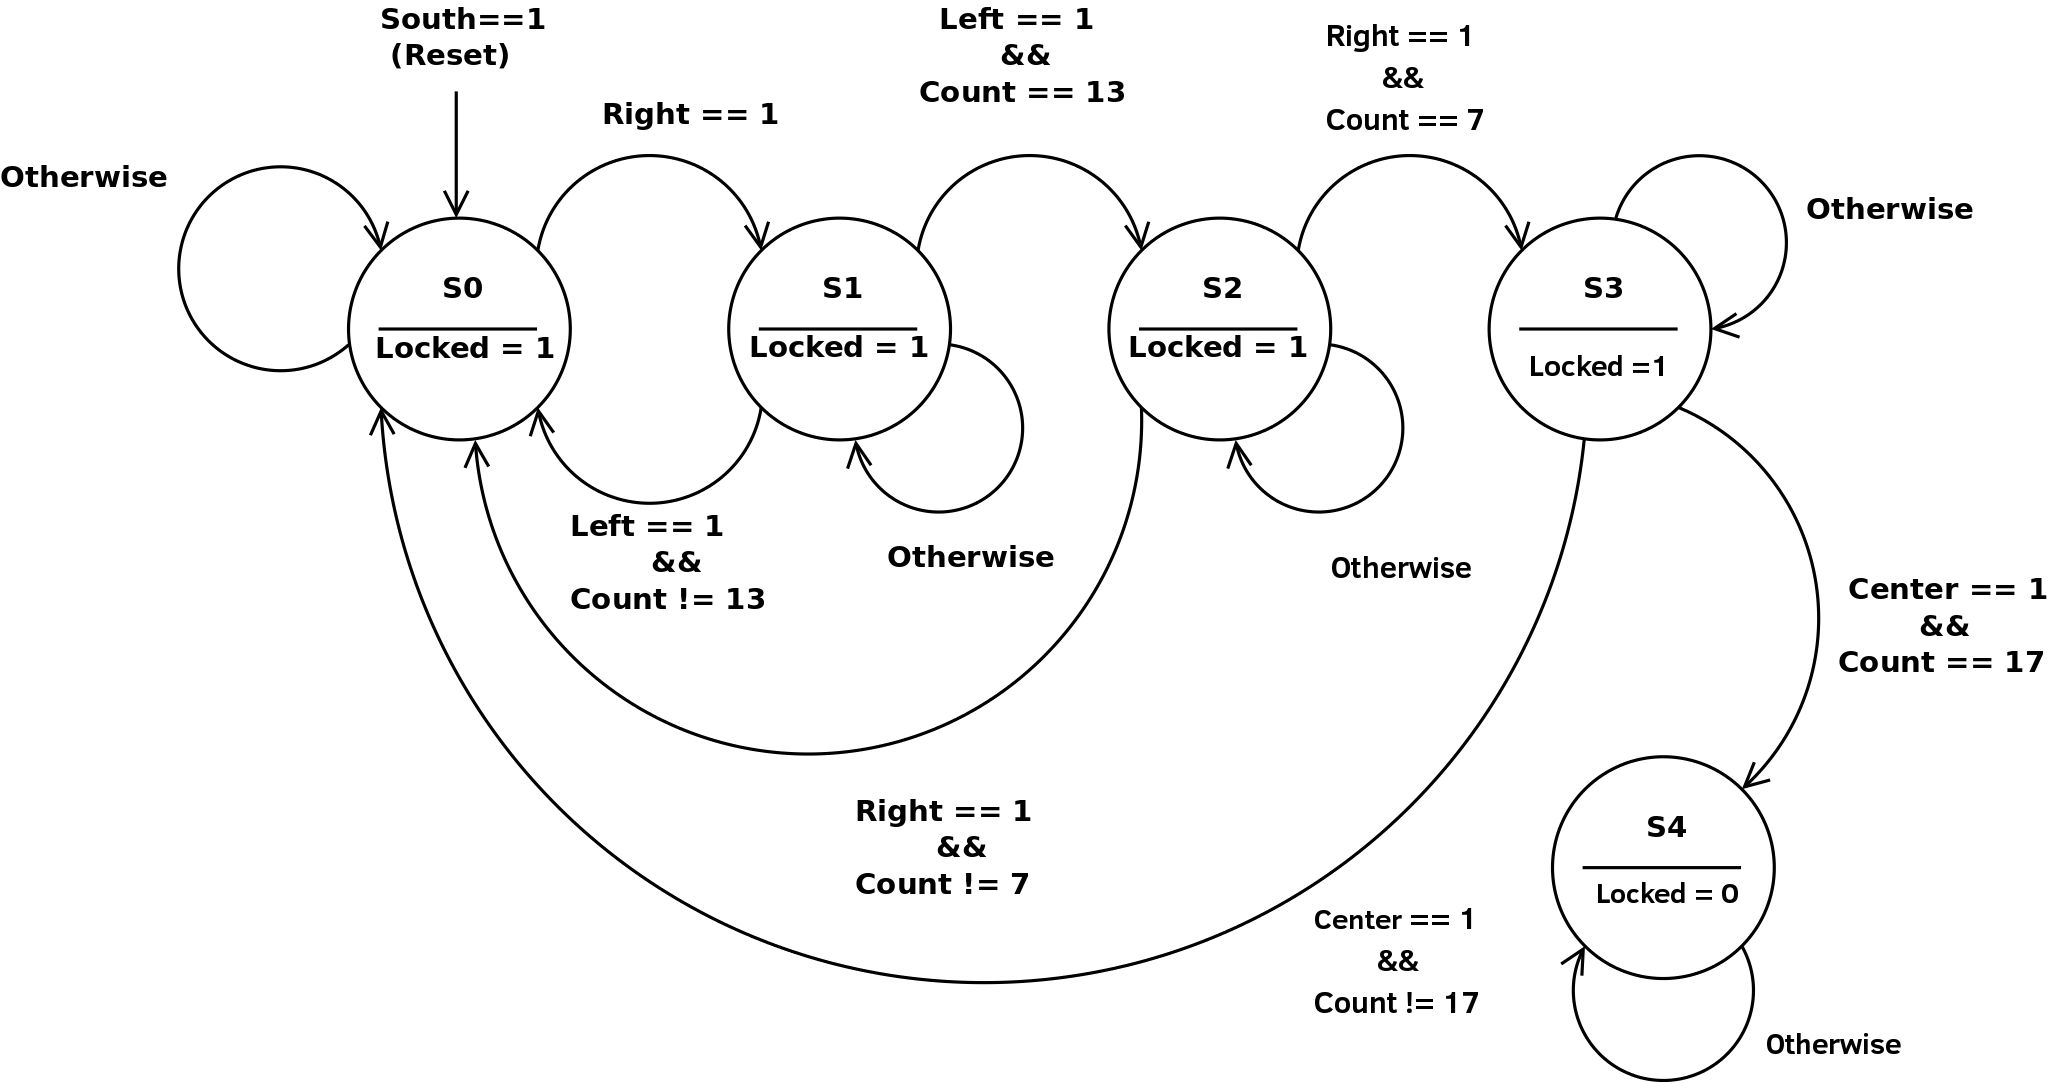
\includegraphics[scale=.21]{AutomaEdit.png}
    \caption{\textit{Rotary Combination-Lock State Diagram}}
  \end{center}
\end{figure}

Below is the Verilog code for the aforementioned Rotary Combination-Lock state diagram that was tested against the appropriate test bench.

\lstinputlisting[language=Verilog,,caption=Combination Lock FSM]{../code/combination_lock_fsm1.v}

For the $2^{\text{nd}}$ part of \textbf{Experiment 1}, the top level module was designed. The top level module is a 0-to-19 Up/Down Counter. This module keeps track of the position of the rotary knob located on the FBGA board. The module below was designed with behavioral Verilog and then tested against the appropriate test bench.

\lstinputlisting[language=Verilog,,caption=Up/Down Counter]{../code/up_down_counter1.v}

\hspace{-15pt}\textbf{Experiment 2}

In the next part of the lab, the previously simulated modules were integrated with a given rotary encoder and LCD driver modules into a top-level module. The rotary combination lock module was set as the top level module. The other modules are as follows: "rotary\_combination\_lock.ucf" (the UCF for the top-level module), "synchronizer.v" (the synchronizer module for the asynchronous inputs), "lcd\_driver.v" (the driver module for the character LCD screen), and "rotary\_encoder\_module.v" (the quadrature decoding module). These modules are below.

\lstinputlisting[language=Verilog,,caption=Rotary Combination Lock Top Level Module]{../code/rotary_combination_lock.v}
\lstinputlisting[language=Verilog,,caption=Rotary Combination Lock UCF File]{../code/rotary_combination_lock.ucf}
\lstinputlisting[language=Verilog,,caption=Synchronizer Module]{../code/synchronizer.v}
\lstinputlisting[language=Verilog,,caption=LCD Driver Module]{../code/lcd_driver.v}
\lstinputlisting[language=Verilog,,caption=Rotary Encoder Module]{../code/rotary_encoder_module.v}

The modules were then synthesized onto the FBGA board and tested. 

In order to add a $4^{\text{th}}$ digit (17), the following changes were made to the combination lock Verilog code. 

\lstinputlisting[language=Verilog,,caption=Combination Lock FSM]{../code/combination_lock_fsm2.v}

This module was then synthesized, along with all the rest, onto the FBGA board.

\section*{Results}

\textbf{Experiment 1}

Below are the results of the the tests as well as the waveform for the combination lock FSM Verilog design.

\newpage

\begin{figure}[h]
  \begin{center}
    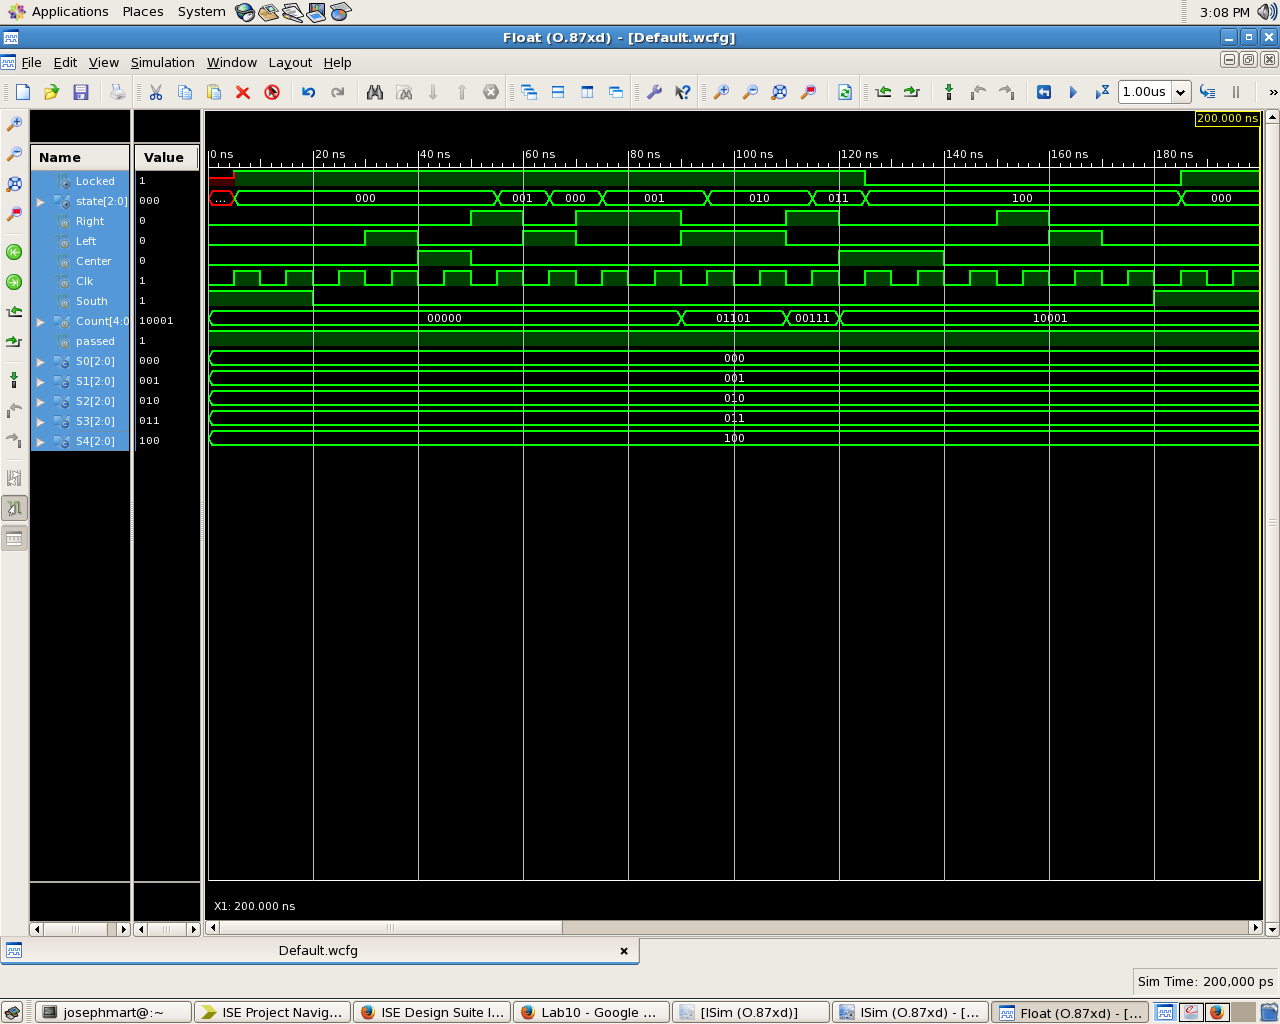
\includegraphics[scale=.1]{Exp1WaveForm.png}
    \caption{\textit{Combination Lock FMS Waveform}}
  \end{center}
\end{figure}

\begin{figure}[h]
  \begin{center}
    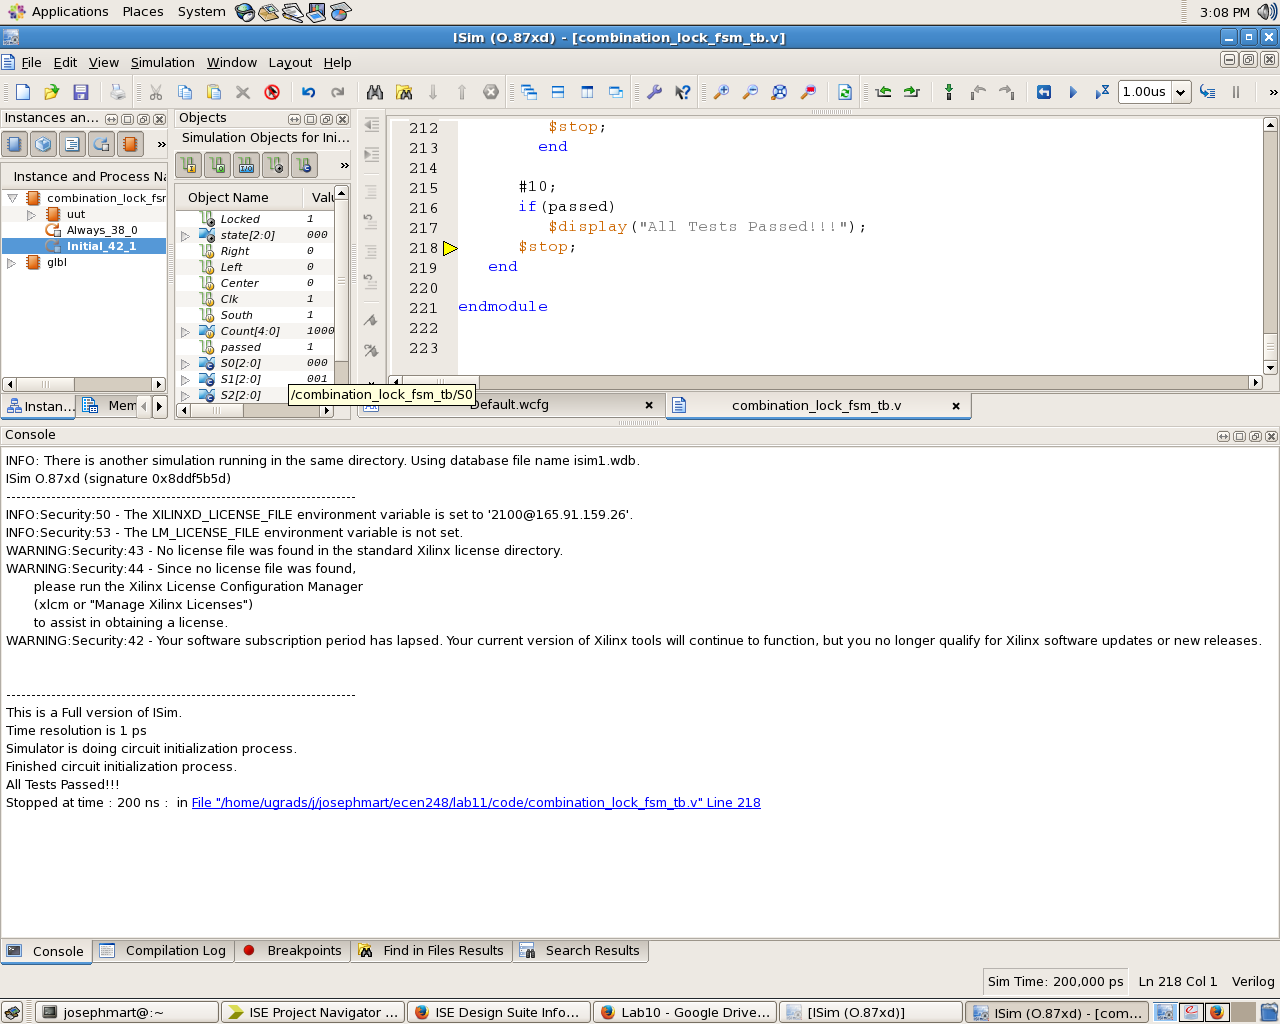
\includegraphics[scale=.1]{ExpTestResults.png}
    \caption{\textit{Combination Lock FMS Test Results}}
  \end{center}
\end{figure}

\newpage

\begin{figure}[h]
  \begin{center}
    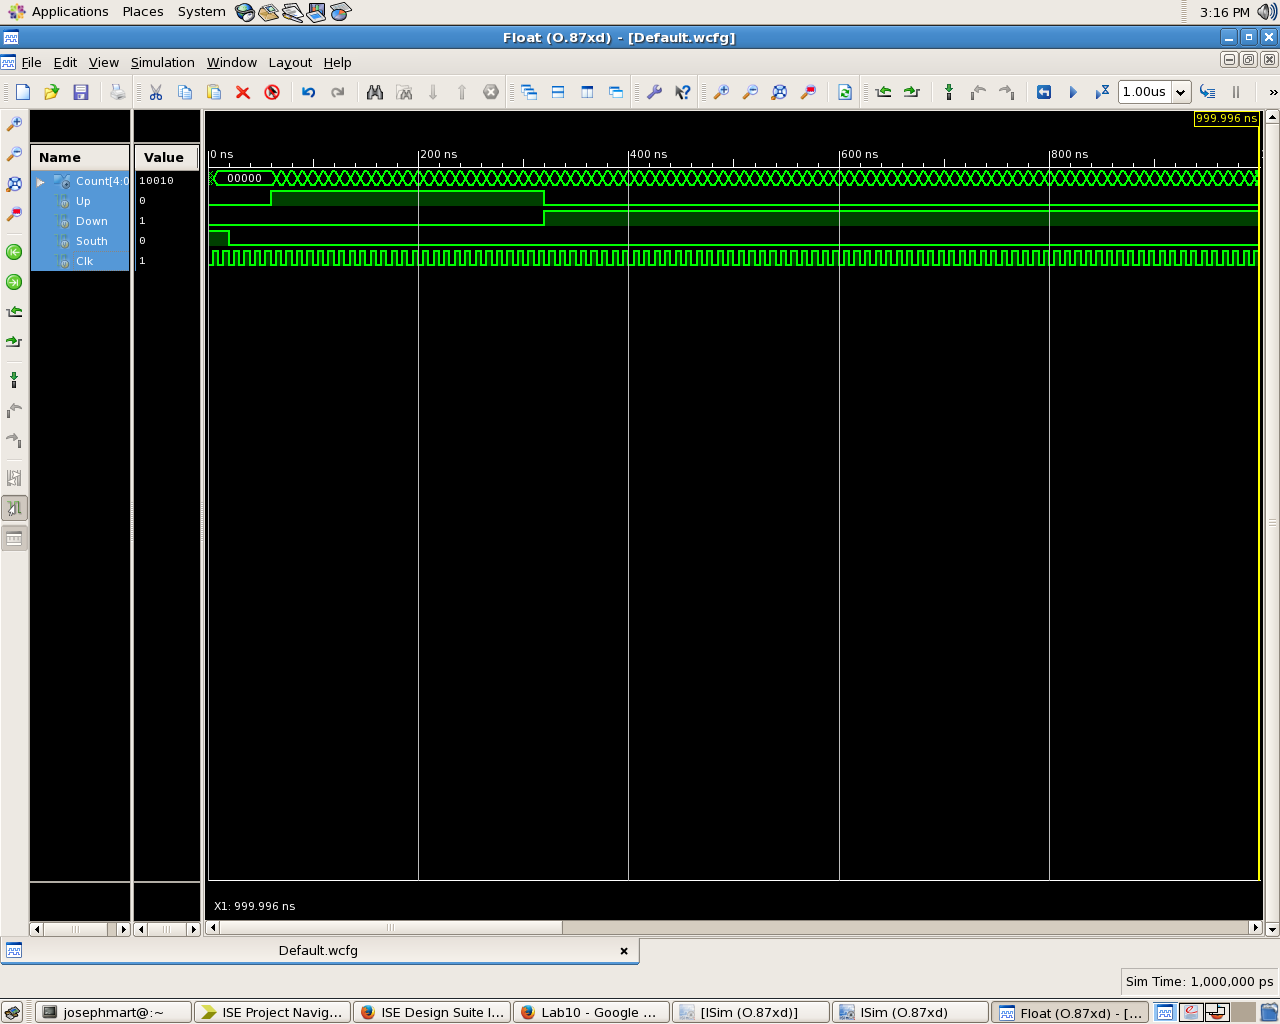
\includegraphics[scale=.1]{UpDownCountWaveForm.png}
    \caption{\textit{Up/Down Counter Waveform}}
  \end{center}
\end{figure}

\begin{figure}[h]
  \begin{center}
    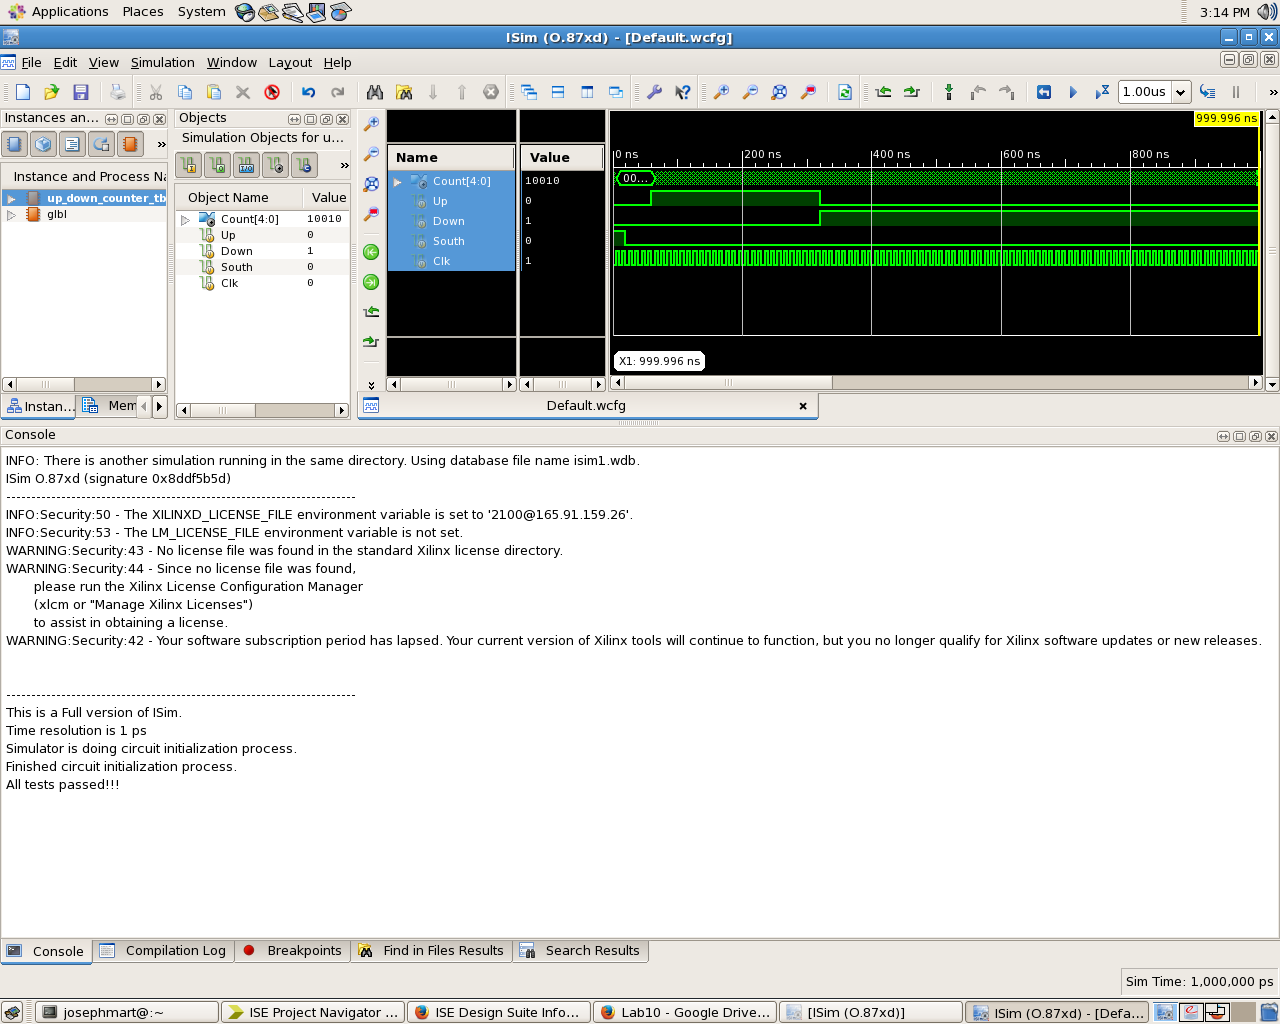
\includegraphics[scale=.1]{UpDownCountTests.png}
    \caption{\textit{Up/Down Counter Test Results}}
  \end{center}
\end{figure}


\section*{Conclusion}

  \hspace{15pt}In conclusion, this lab allowed me to learn more about Verilog and circuit design. This lab showed me how through the iteration of modules and through synthesizing, an everyday use object (combination lock) can be created, with a little help, by a simple sophomore engineer.


\section*{Questions}

\begin{enumerate}
  \item \textbf{Include the source code with comments for all modules you simulated and/or implemented in lab. You do not have to include test bench code that was provided! Code without comments will not be
accepted!}

  \item \textbf{Include screenshots of all waveforms captured during simulation in addition to the test bench console output for each test bench simulation.}

  \item \textbf{Answer all questions throughout the lab manual.}
  
  \item \textbf{A possible attack on your combination-lock is a brute-force attack in which every possible input combination is tried. Given the original design with a combination of three numbers between 0 and 19, how many possible input combinations exist? How about for the modified design with a combination of four numbers?}
\end{enumerate}

\section*{Student Feedback}

\begin{enumerate}
  \item \textbf{What did you like most about the lab assignment and why? What did you like least about it and why?}
  \vspace{10pt}

  \item \textbf{Were there any section of the lab manual that were unclear? If so, what was unclear? Do you have any suggestions for improving the clarity?}
  \vspace{10pt}

  \item \textbf{What suggestions do you have to improve the overall lab assignment?}
  \vspace{10pt}

\end{enumerate}

\ifx
\begin{thebibliography}{1}
\bibitem{Verilog} Charles Kime \& Thomas Kaminski  \emph{Logic and Computer Design Fundamentals} \\ \hspace{15pt}\textit{http://www.cs.bilkent.edu.tr/~will/courses/CS223/Verilog/LCDF3_Verilog_Ch_4.pdf}
\end{thebibliography}

\section*{Attachments}
%Make sure to change these
Lab Notes, HelloWorld.ic, FooBar.ic
%\fi %comment me out

\begin{thebibliography}{9}
\bibitem{Verilog} Charles Kime & Thomas Kaminski  \emph{Logic and Computer Design Fundamentals} \textit{http://www.cs.bilkent.edu.tr/~will/courses/CS223/Verilog/LCDF3_Verilog_Ch_4.pdf}
\end{thebibliography}

%How to cite
Put your Problem statement here! Example of a Citation\cite[p.219]{Robotics}. Here's Another Citation\cite{Flueck}
\fi
\end{document}
